\documentclass[usenames,dvipsnames,pdftex,unicode,hidelinks]{beamer}
  \usepackage{cmap}
  \usepackage[T2A]{fontenc}
  \usepackage[utf8]{inputenc}
  \usepackage[english,russian]{babel}
  \usepackage{wasysym}
  \usepackage{mathtext} % для кириллицы в формулах
    \DeclareSymbolFont{T2Aletters}{T2A}{cmr}{m}{it} % кириллица в формулах курсивом

  \usepackage{tikz}
    \usetikzlibrary{positioning,fit,shapes}
  \graphicspath{{../img/}{../../img/}}

  % Русификация definition
  \newtheorem{ru-def}{Определение}
  \renewenvironment{definition}{\begin{ru-def}}{\end{ru-def}}

  % Начало раздела с показом его заголовка на весь кадр
  \newcommand{\splashsection}[1]{
    \section{#1}
    \begin{frame}[plain]
      \begin{center}
        \huge #1
      \end{center}
    \end{frame}
  }

  % add frame number to footline
  \let\oldmacro\insertshorttitle
  \renewcommand*\insertshorttitle{
    \insertshortauthor : % Добавляем автора, которого нет в Szeged
    \oldmacro\hfill
    \insertframenumber\,/\,\inserttotalframenumber
  }

  % hide navigation symbols
  \beamertemplatenavigationsymbolsempty

  \usetheme{Szeged}%{Warsaw}
  \usecolortheme{albatross}
  \usefonttheme{structurebold}
  \useinnertheme{rounded}
  % Патчим некоторые цвета
  \setbeamertemplate{background canvas}[vertical shading][bottom=black!60!blue,top=black!80!blue]
  \setbeamercolor{block title}{bg=black!50!Blue}
  \setbeamercolor{block body}{bg=black!80!blue}

  \setbeamercovered{transparent}

\title[Чёрные дыры]{
  \texorpdfstring{
    %\newcounter{cntOpacity}
    \begin{tikzpicture}[scale=0.9]
      \foreach \x in {0, ..., 6}
        \shade[shading=ball, ball color=black] (2.5*\x - 0.15*\x*\x, 0) circle (1-\x*0.15);
    \end{tikzpicture}
    \\
  }{}Чёрные дыры
}
\author[Иван Новиков]{
  Новиков Иван Александрович\texorpdfstring{
    \\
    \vspace{0.3cm}
    \small 1 курс магистратуры ФТФ, напр. Физика
  }{
    - КубГУ, ФТФ, 1 курс магистратуры
  }
}

\institute{Кубанский Государственный Университет}

\date{ 29 мая 2013 г. }

\begin{document}
  
  \begin{frame}[plain]
    \titlepage
  \end{frame}

  \splashsection{Введение}
  \subsection{Область применения термина}

  \begin{frame}{Астрономия}
    \begin{center}
      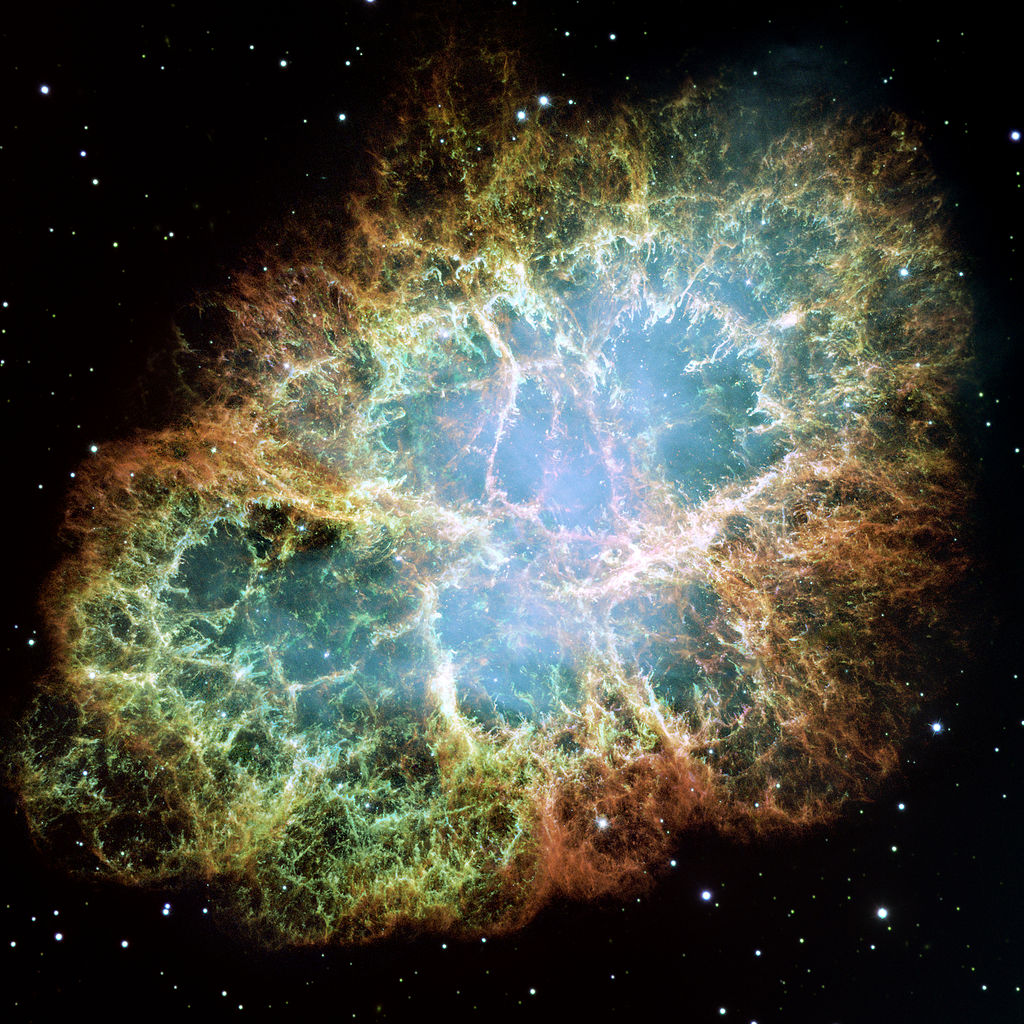
\includegraphics[height=0.8\textheight]{crab-nebula}
     \end{center}
  \end{frame}

  \begin{frame}{Судьбы звёзд \small (что может быть пафоснее)}
    \begin{enumerate}
      \item<1-> $\boldsymbol{M} < 1.4 \cdot M_{\sun}$\\
        $\Rightarrow$ белый карлик {\small + протопланетная туманность}
        \begin{center}
          \only<1>{ 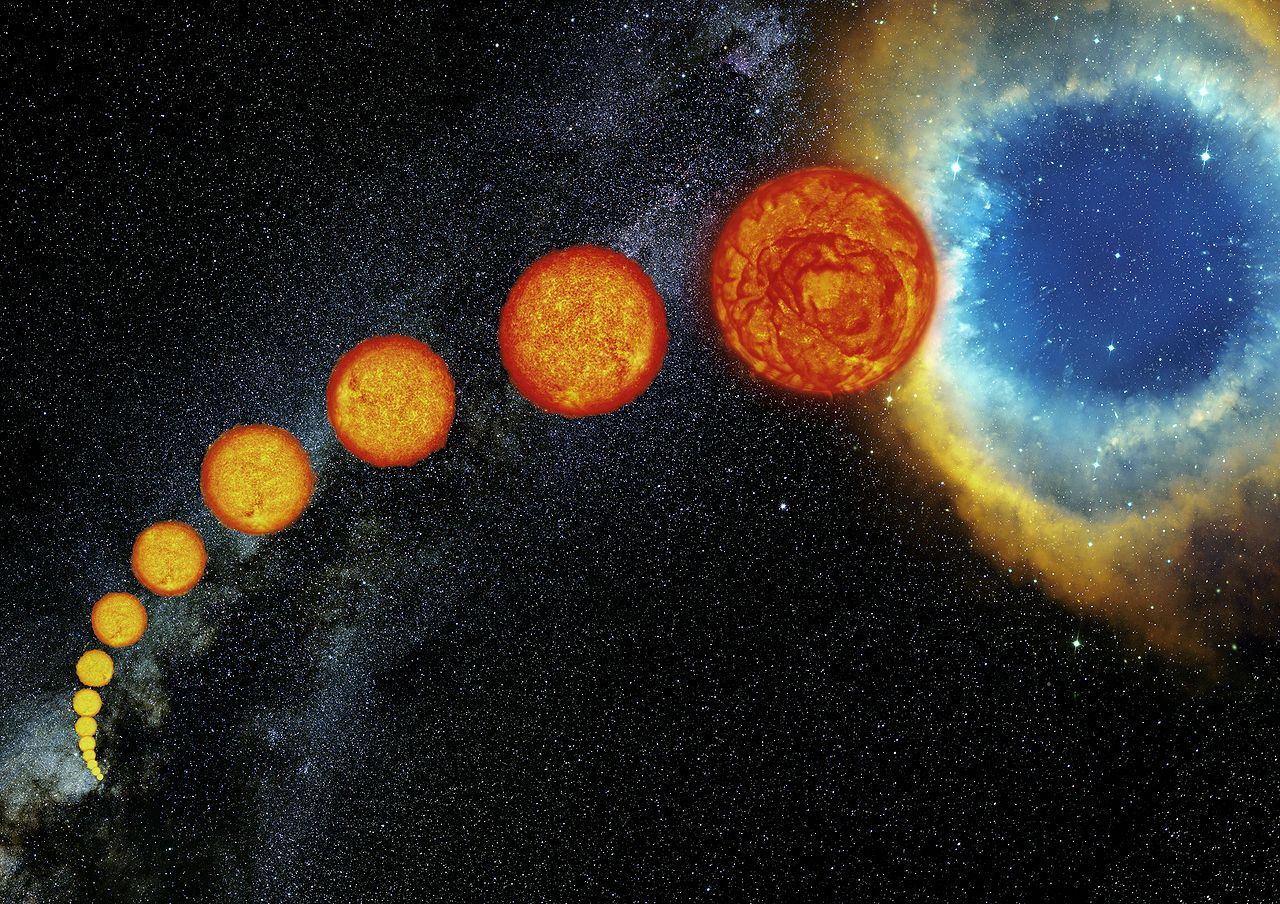
\includegraphics[height=0.4\textheight]{sun-evolution}  }
        \end{center}
      \item<2-> $1.4 \cdot M_{\sun} < \boldsymbol{M} < 10 \cdot M_{\sun}$\\
        $\Rightarrow$ нейтронная звезда {\small + туманность от сверхновой}
        \begin{center}
          \only<2>{ 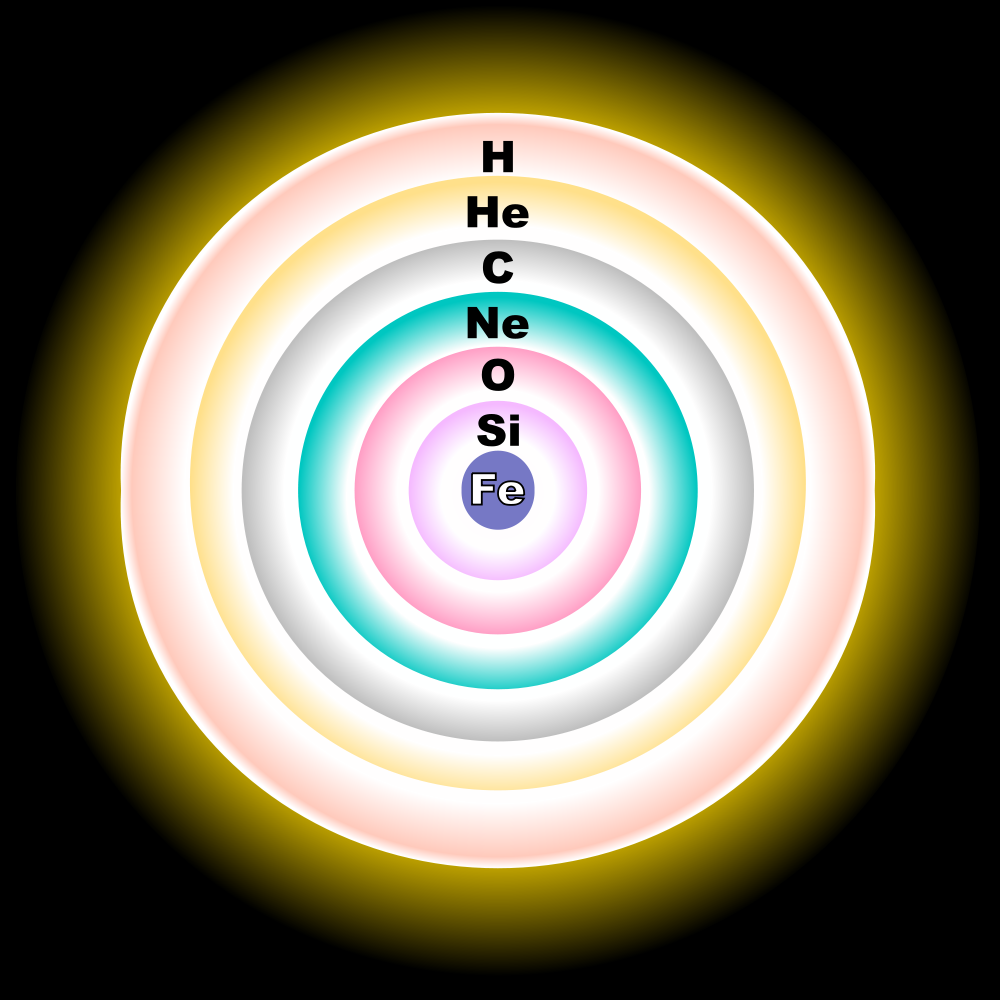
\includegraphics[height=0.4\textheight]{evolved-massive-star}  }
        \end{center}
      \item<3-> $10 \dots 20 \cdot M_{\sun} < \boldsymbol{M} $\\
        $\Rightarrow$ ЧЁРНАЯ ДЫРА
        \begin{center}
          \only<3>{ 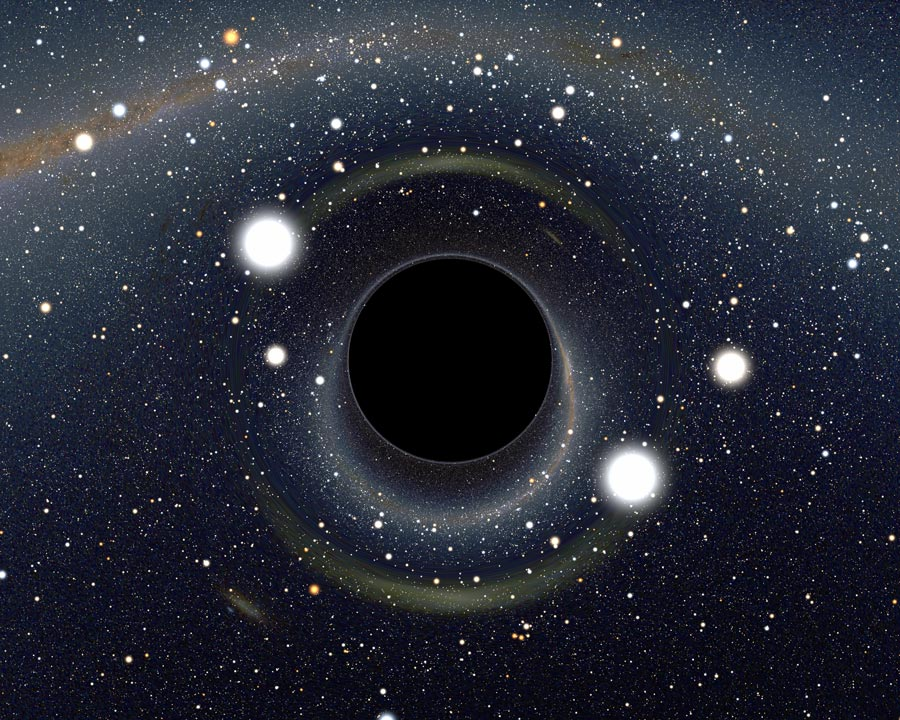
\includegraphics[height=0.4\textheight]{black-hole}  }
        \end{center}
    \end{enumerate}
  \end{frame}

  \subsection{Определение термина}

  \begin{frame}{Понятие чёрной дыры}
    \begin{definition}
      \alert{ЧЁРНАЯ ДЫРА}~--- область пространства, в которой гравитационное притяжение настолько
      сильно, что ни вещество, ни излучение не могут эту область покинуть.
    \end{definition}

    \begin{center}
      \begin{tikzpicture}[scale=3, transform shape]
        \node {$ v_2 > c $};
      \end{tikzpicture}
    \end{center}

    \begin{definition}
      Границу области, за которую не выходит свет, называют \alert{горизонтом событий}, или
      просто <<горизонтом>> чёрной дыры.
    \end{definition}
  \end{frame}

  \begin{frame}{Вывод второй космической скорости}
    \begin{columns}[c]
      \begin{column}{0.25\textwidth}
        \begin{center}
        \begin{tikzpicture}
          \tikzstyle{planet} = [circle, shade=ball, ball color=cyan, text=black, minimum size=2cm]
          \tikzstyle{ship} = [circle, text=black, draw=black, shade=ball, ball color=white]
          \tikzstyle{noship} = [circle, shade=ball, ball color=white, fill opacity = 0.2, text=white, draw=white, loosely dashed]
          \tikzstyle{energy} = [font=\footnotesize]
          \node[planet] (Planet) {M};
          \only<1>{
            \node[ship] (Ship) at (Planet.north) {m};
            \node[noship] (Ship2) [above=3cm of Ship] {m};
            \draw[->, dashed, gray, very thick] (Ship) -- (Ship2);
          }
          \only<2->{
            \node[noship] (Ship4) at (Planet.north) {m};
            \node[ship] (Ship3) [above=3cm of Ship4] {m};
            \draw[->, dashed, gray, very thick] (Ship3) -- (Ship4);

            \node<3->[energy, below] at (Ship3.south) { $E = T + U = 0$ };
            \node<3->[energy, above] at (Ship4.north) { $E = \frac{mv_2^2}{2} - G\frac{mM}{R}$ };
          }
        \end{tikzpicture}
        \end{center}
      \end{column}
    \begin{column}{0.75\textwidth}
        \begin{itemize}
          \item<1-> Какая min $v$ нужна, чтобы улететь на $\infty$?
          \item<2-> \alert{ИЛИ:} Какую $v$ будет иметь, упав с $\infty$?
          \item<3-> Закон сохранения энергии:
            \[
              \frac{mv_2^2}{2} - G\frac{mM}{R} = 0
            \]
          \item<4-> Решая относительно $v_2$:
            \[
              v_2 = \sqrt{2G\frac{M}{R}}
            \]
        \end{itemize}
      \end{column}
    \end{columns}
  \end{frame}

  \begin{frame}{Гравитационный радиус в классической механике}
    \begin{itemize}
      \item<1-> Итак, вторая космическая скорость
        \[
          v_2 = \sqrt{2G\frac{M}{R}}
        \]
      \item<2-> Подставляя условие $v_2 < c$:
        \[
          c^2 < v_2^2 = 2G\frac{M}{R}
        \]
      \item<3-> Получаем для данной массы $M$ такой радиус, при котором ничто не сможет улететь:
        \[
          \boxed{
            R < 2G\frac{M}{c^2}
          }
        \]

      \begin{tikzpicture}[overlay]
        \node<3->[shift={(-4cm, 1cm)}] at (current page.south east) {
          
\includegraphics[width=2.5cm]{muahaha}
        };
      \end{tikzpicture}
    \end{itemize}
  \end{frame}

  \splashsection{История}

  \begin{frame}{Основные этапы}
    \begin{itemize}
      \item<1> $1784\dots1915$\\--- Дж.\,Мичелл, расчёт массы для недоступного наблюдению объекта 
      \item<2> $1915\dots1975$\\--- К.\,Шварцшильд, стационарное решение уравнений Эйнштейна (ОТО)
      \item<3> $1975\dots$\\--- C.\,Хокинг, идея об излучении чёрных дыр
    \end{itemize}
  \end{frame}

  \subsection{<<Чёрная звезда>> Мичелла}
    
  \begin{frame}{Джон Мичелл}
    \begin{columns}[t]
      \begin{column}{0.25\textwidth}
        \begin{center}
          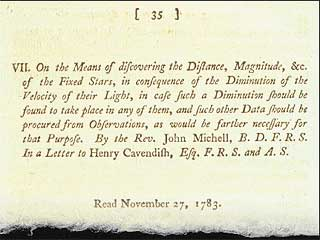
\includegraphics[width=\textwidth]{michell-paper-001}\\
          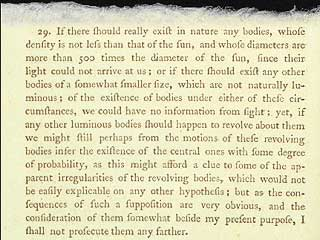
\includegraphics[width=\textwidth]{michell-paper-002}

          \textbf{1724--1793}
        \end{center}
      \end{column}
      \begin{column}{0.75\textwidth}
        \begin{itemize}
          \item Английский геофизик и астроном, занимался оптикой и гравитацией
          \item В \alert{1784} высказал идею небесного тела, невидимого из-за того, что $v_2 > c$
          \item Рассчитал, что таковым будет тело с $R = 100\cdot R_{\sun}$ и $\rho = \rho_{\sun}$
          \item Сообщил о своей идее Лондонскому Королевскому Обществу.
        \end{itemize}
        \begin{center}
          \vspace{5mm}
          
\includegraphics[width=1cm]{britain}
        \end{center}
      \end{column}
    \end{columns}
  \end{frame}
    
  \begin{frame}{Пьер-Сим\'{о}н Лаплас}
    \begin{columns}[t]
      \begin{column}{0.25\textwidth}
        \begin{center}
          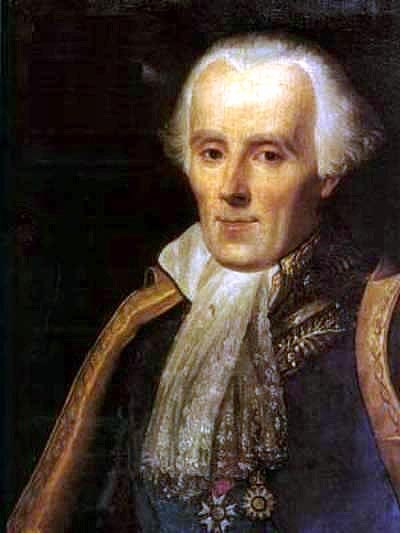
\includegraphics[width=\textwidth]{laplace}\\
          \textbf{1749--1827}
        \end{center}
      \end{column}
      \begin{column}{0.75\textwidth}
        \begin{itemize}
          \item Выдающийся французский математик, физик и астроном
          \item Известен работами в области небесной механики, дифференциальных уравнений, один из создателей теории вероятностей
          \item \alert{Включил идеи Мичелла} в свой труд «Exposition du Systeme du Monde»
          \item Потом убрал, но благодаря ему эта мысль \alert{получила известность}
        \end{itemize}
        \begin{center}
          
\includegraphics[width=1cm]{france}
        \end{center}
      \end{column}
    \end{columns}
  \end{frame}

  \begin{frame}{После Мичелла}
    \begin{itemize}
      \item<1-> Поначалу идея \alert{не вызывала интереса}: в классической механике скорость света не
        имеет фундаментального значения
      \item<2-> В 1905 году Эйнштейн создаёт СТО на основе концепций Лоренца и Пуанкаре: в новой
        механике $c$~--- предельная скорость
      \item<3-> \alert{НО:} тогда и Ньютоновская теория тяготения, из которой мы вывели чёрные дыры,
        тоже не верна \emph{(Ooops!)}
      \item<4-> Нас спасёт \alert{общая теория относительности!} (ОТО)\\
        \emph{Браво, Эйнштейн!}
    \end{itemize}
    \begin{tikzpicture}[overlay]
      \node<4-> at (current page.south) {
        
\includegraphics[width=1.5cm]{applause}
      };
    \end{tikzpicture}
  \end{frame}

  \subsection{Чёрные дыры в общей теории относительности}

  \begin{frame}{Уравнения Эйнштейна}
    \begin{itemize}[<+->]
      \item (Было) Теория гравитации Ньютона:
        \[
          F = G \frac{Mm}{r^2}
        \]
      \item (Стало) Теория гравитации Эйнштейна:
         \[
           R_{ab} - \frac{R}{2}  g_{ab} + \Lambda g_{ab} = \frac{8 \pi G}{c^4} T_{ab}
         \]
    \end{itemize}
    \begin{flushright}
      \only<1>{
\includegraphics[height=3cm]{cereal-guy-1}}
      \only<2>{
\includegraphics[height=3cm]{cereal-guy-2}}
    \end{flushright}
    
  \end{frame}

  \begin{frame}{Карл Шварцшильд}
    \begin{columns}[t]
      \begin{column}{0.25\textwidth}
        \begin{center}
          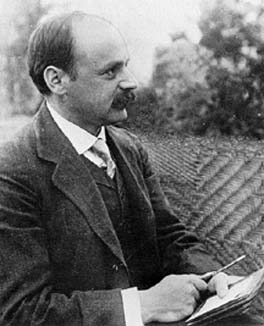
\includegraphics[width=\textwidth]{schwarzschild}\\
          \textbf{1873--1916}
        \end{center}
      \end{column}
      \begin{column}{0.75\textwidth}
        \begin{itemize}
          \item Немецкий астроном и физик, профессор Гёттингенского университета, директор астрофизической обсерватории в~Потсдаме
          \item Ещё до появления ОТО исследует возможность того, что пространство является неевклидовым
          \item Заболел на фронте смертельной болезнью, в госпитале написал две статьи по ОТО и
            фундаментальную работу по квантовой теории Бора~--- Зоммерфельда

        \end{itemize}
        \begin{center}
          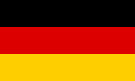
\includegraphics[width=1cm]{germany}
        \end{center}
      \end{column}
    \end{columns}
  \end{frame}

  \begin{frame}{Решение Шварцшильда}
    \begin{itemize}[<+->]
      \item Изолированная невращающаяся, незаряженная и не испаряющаяся чёрная дыра
      \item Горизонт событий — это сфера, радиус которой называется гравитационным радиусом или радиусом Шварцшильда
      \[
        \boxed{
          r_s = 2G\frac{M}{c^2}
        }
      \]
      \item \alert{Совпадает} по величине с классическим результатом!
      \item Но причина другая: сильное искривление\\ метрики пространства-времени
    \end{itemize}
    \vfill
    \begin{tikzpicture}[overlay]
      \node<4->[shift={(-3cm, 0.7cm)}] at (current page.south east) {
        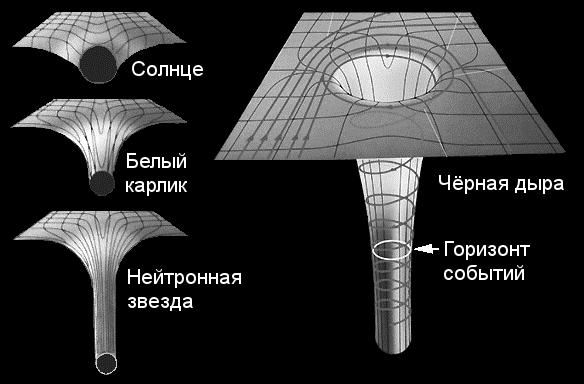
\includegraphics[width=3.7cm]{space-warp}
      };
    \end{tikzpicture}
  \end{frame}

  \begin{frame}{Радиус Шварцшильда}
    Значения $r_s$ для типичных масс:
    \begin{eqnarray*}
      M = M_{\text{земли}} = 5,972\cdot 10^{24} \text{ кг} & \Rightarrow r_s = 9 \text{ мм} \\
      M = M_{\sun} = 1,989\cdot 10^{30} \text{ кг} & \Rightarrow r_s = 3 \text{ км}
    \end{eqnarray*}
    \begin{block}{Вывод}<2->
      Вещество в чёрной дыре должно быть \alert{очень плотным}.
    \end{block}
  \end{frame}

  \begin{frame}{Стивен Хокинг}
    \begin{columns}[t]
      \begin{column}{0.25\textwidth}
        \begin{center}
          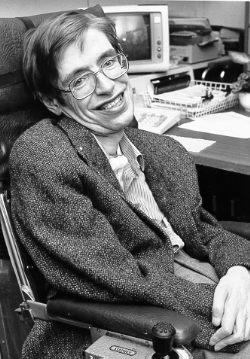
\includegraphics[width=\textwidth]{hawking}\\
          \textbf{1942--...}
        \end{center}
      \end{column}
      \begin{column}{0.75\textwidth}
        \begin{itemize}
          \item Один из наиболее влиятельных и известных физиков-теоретиков и космологов
          \item Применил термодинамику к описанию чёрных дыр
          \item Разработал в 1975 г. теорию о том, что чёрные дыры «испаряются»:
            \\ \alert{излучение Хокинга}
          \item В 2004 году показал, что чёрная дыра искажает
            проглоченную информацию, но не разрушает её бесследно.
        \end{itemize}
        \begin{center}
          
\includegraphics[width=1cm]{britain}
        \end{center}
      \end{column}
    \end{columns}
  \end{frame}

  \begin{frame}{Что дальше?}
    \begin{itemize}
      \item В теории ещё много открытых вопросов...
        \begin{itemize}
          \item Так всё-таки пропадает ли в них информация?
          \item Какова структура вращающихся чёрных дыр?
          \item Как влияет излучение Хокинга на горизонт событий?
          \item Могут ли они помочь путешествовать\\ в пространстве и времени?
          \item Что будет, если две чёрные дыры столкнутся?
          \item Чем заканчивается испарение чёрной дыры?
        \end{itemize}
      \item А пока~--- перейдём к практике!
    \end{itemize}
  \end{frame}

  \splashsection{Практика}

  \subsection{Наблюдение чёрных дыр}

  \begin{frame}{Как увидеть чёрную дыру?}
    \begin{itemize}
      \item<1-> Можно рассчитать каким-либо способом массу и радиус объекта и понять, является ли он
        чёрной дырой
        \vspace{3mm}
      \item<1-> Но можно ли её именно \alert{увидеть}?
        \vspace{3mm}
      \item<2-> Напрямую~--- всё-таки нет, но косвенно~--- да!
    \end{itemize}
  \end{frame}

  \begin{frame}{Гравитационное линзирование}
    \begin{definition}
      {
        \footnotesize
        \alert{Гравитационная линза}~--- массивное тело, искривляющее своим гравитационным полем
        направление распространения электромагнитного излучения, подобно тому, как искривляет
        световой луч обычная линза.
      }
    \end{definition}
    \begin{center}
      \begin{tikzpicture}[scale=0.9, transform shape]
        \tikzstyle{object} = [star, star points=4, star point ratio=2, draw=white, fill=yellow!20!white]
        \tikzstyle{lens}   = [circle, shade=ball, ball color=black, minimum size=7mm, text=white]
        \tikzstyle{planet} = [circle, shade=ball, ball color=cyan, minimum size=4mm, text=black]
        \tikzstyle{ray}    = [->, yellow!20!white, thick]
        \tikzstyle{imaginary} = [loosely dashed, fill opacity = 0.4]

        \node[object] (Star)  at (0,0) {};
        \node[lens]   (Lens)  at (4,0) {M};
        \node[planet] (Earth) at (8,0) {};

        \draw[ray] (Star) to [out=10,in=170] (Earth);
        \draw[ray] (Star) to [out=-10,in=-170] (Earth);

        \visible<2->{
          \node[imaginary, object, rotate=-20] (Star1) at (0,  1.5) {};
          \node[imaginary, object, rotate= 20] (Star2) at (0, -1.5) {};
          \draw[imaginary, ray] (Star1) -- (Earth);
          \draw[imaginary, ray] (Star2) -- (Earth);
        }
      \end{tikzpicture}

      \uncover<2->{
        \footnotesize
        Изображение объекта нам может казаться раздвоенным, если между нами и объектом~--- очень
        массивное тело: галактика или... чёрная дыра?
      }
    \end{center}
  \end{frame}

  \begin{frame}{Чёрная дыра как гравитационная линза}

    {
      \footnotesize
      Что-то подобное мы бы увидели, если бы смогли подлететь к чёрной дыре достаточно
      близко (результат компьютерного моделирования):
      \begin{center}
        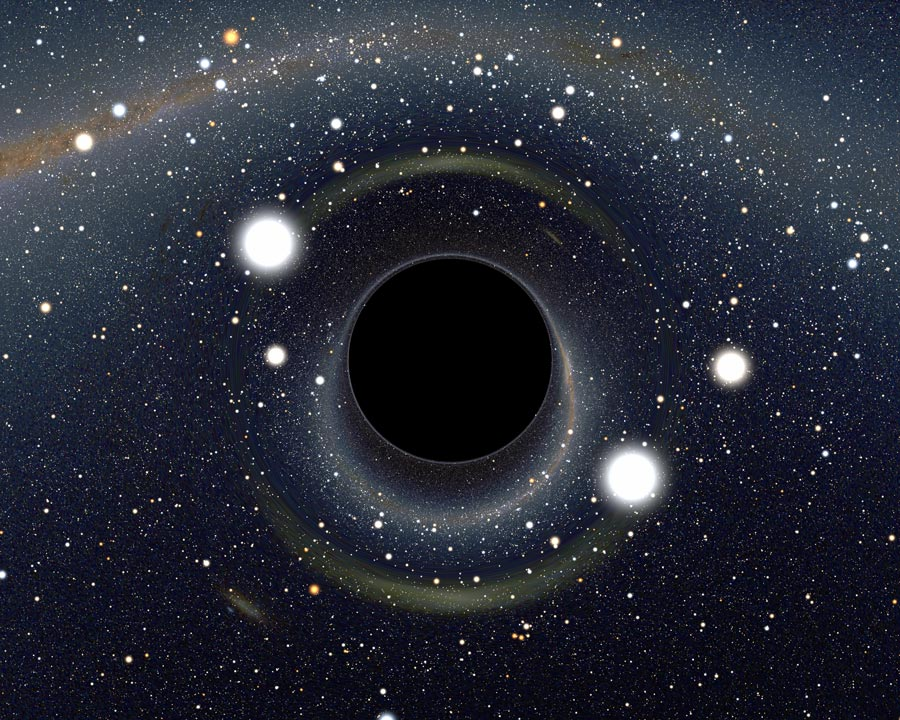
\includegraphics[height=0.6\textheight]{black-hole}
      \end{center}
      Виден эффект раздвоения, искажение формы, <<Кольцо Эйнштейна>>~---
      уменьшенное отражение окружающей галактики вокруг чёрной дыры
    }
  \end{frame}

  \begin{frame}{Аккреция}
    \begin{definition}
      \alert{Аккр\'{е}ция} (лат. accr\={e}ti\={o} «приращение, увеличение»)~--- процесс падения
      вещества на космическое тело из окружающего пространства
    \end{definition}

    \begin{itemize}
      \item Из-за орбитального движения вещество падает не прямо, а~вращаясь по кеплеровским
        орбитам и образуя \alert{аккреционный диск}
      \item<2-> При поглощении вещества \textbf{чёрной дырой} аккреционный диск сильно \alert{излучает}
        в~рентгеновском диапазоне\\ \emph{(не путать с излучением Хокинга!)}
    \end{itemize}
  \end{frame}

  \begin{frame}{Наблюдение аккреции чёрной дырой}

    {
      \small
      В апреле 2013 опубликованы\footnote{M. Niko\l ajuk, R. Walter Tidal disruption of a super-Jupiter by a massive black hole // Astronomy and Astrophysics. — 2013. — Т. 552. — P. A75.}
      наблюдения со спутника INTEGRAL
      \begin{center}
        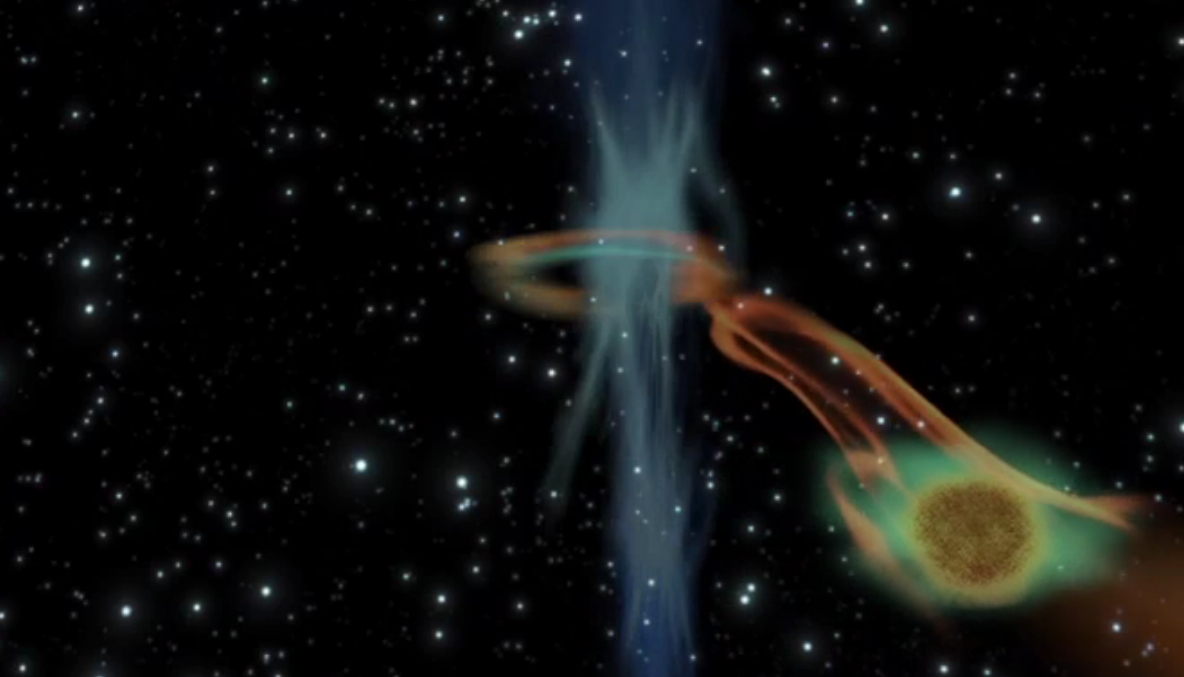
\includegraphics[height=0.4\textheight]{accretion}
      \end{center}
      Чёрная дыра в центре галактики NGC 4845 <<съела>> поверхность гигантской планеты-сироты,
      при этом светимость галактики в рентгеновском диапазоне возросла в 100 раз
    }
  \end{frame}

  \subsection{Местонахождение чёрных дыр}

  \begin{frame}{Где мы можем их встретить?}
    \begin{itemize}
      \item Итак, более или менее понятно, \alert{как} искать чёрные дыры
        \vspace{1cm}
      \item Так \alert{где} же они были найдены к настоящему моменту?
    \end{itemize}
  \end{frame}

  \begin{frame}{Кандидаты в чёрные дыры}
    \begin{itemize}
      \item Наилучшие кандидаты~--- ядра галактик:
        \begin{itemize}
          \item<2-> Туманность Андромеды
          \item<2-> Галактика Сомбреро
          \item<2-> NGC 4845, поедающая планету
          \item<3-> И наш \alert{Млечный Путь}~--- тоже!
        \end{itemize}
       \item<4-> Микроквазары~---двойные системы с мощной аккрецией
        \begin{itemize}
          \item<4-> Скорпион X1
          \item<4-> Лебедь X1
        \end{itemize}
        \item<5-> Некоторые другие варианты
    \end{itemize}
  \end{frame}

  \section{}% Заканчиваем раздел "Практика", чтобы заключение, литература, и "спасибо" к нему не относились

  \begin{frame}{Заключение}
    \begin{block}{Выводы}
      \begin{enumerate}
        \item Теория чёрных дыр содержит много запутанных вещей, и понять её чрезвычайно сложно
          \vspace{5mm}
        \item Зато с практикой гораздо проще: уже с современными технологиями можно наблюдать чёрные дыры
          \vspace{5mm}
        \item Наша галактика~--- классная, в ней есть чёрная дыра :)
      \end{enumerate}

    \end{block}
  \end{frame}

  \begin{frame}{Литература}
    \begin{enumerate}
      \item
        \href{https://ru.wikipedia.org/wiki/\%D0\%A7\%D1\%91\%D1\%80\%D0\%BD\%D0\%B0\%D1\%8F_\%D0\%B4\%D1\%8B\%D1\%80\%D0\%B0}{\texttt{https://ru.wikipedia.org/wiki/Чёрная\_дыра}}
        \\(sad, but true)
      \item И.\,Орлов. Космология, или откуда всё взялось и куда потом денется?
        (\url{http://www.slideshare.net/OrlovIO/ss-18715909})
      \item М.\,Каку. Физика невозможного.
    \end{enumerate}
  \end{frame}

  \begin{frame}[plain]
    \begin{center}
      { \Huge Спасибо за внимание! }

      \vspace{1cm}

      Иван Новиков\\
      \url{http://about.me/moonlighter}\\
      \href{mailto:nia.afti@gmail.com}{\nolinkurl{nia.afti@gmail.com} }
      
    \end{center}
  \end{frame}

\end{document}

